\documentclass{ltjbook}
\usepackage{docmute} 
\usepackage{../../myStyle} 
\begin{document}

\chapter{Analysis of Variance with R}
\label{m22_anovaOnR}
So far, we have explained the approach of considering experimental design as a linear model or within the framework of null hypothesis testing.
I would like to collect the topic that I postponed earlier, which stated that detailed calculations will be done with R. Let's learn how the calculations progress, how the results are displayed, and how to interpret the results with exercises using R.
\section{Key Points for Conducting Analysis of Variance in R}
Let's start by launching R. As a quick review, I'll write again about the first step before starting the task.
\paragraph{Starting RStudio}
Please start RStudio. There may be cases where administrator privileges are required, such as when installing packages.
\paragraph{Opening the Project}I think it would be fine to use the same project we created last time. You just need to change the script file in the same folder. Open the project from the menu (File$\to$Open Project), and make sure the project is open, for example, in the top right of RStudio (see Figure \ref{fig::20_01}).
\paragraph{Opening an R Script} 

To write today's code, let's prepare an R script file. Go to \verb|File > New File > R Script| and open a blank R script screen. If a completely blank file opens up, you're good to go.
\begin{figure}[ht]
   \centering
   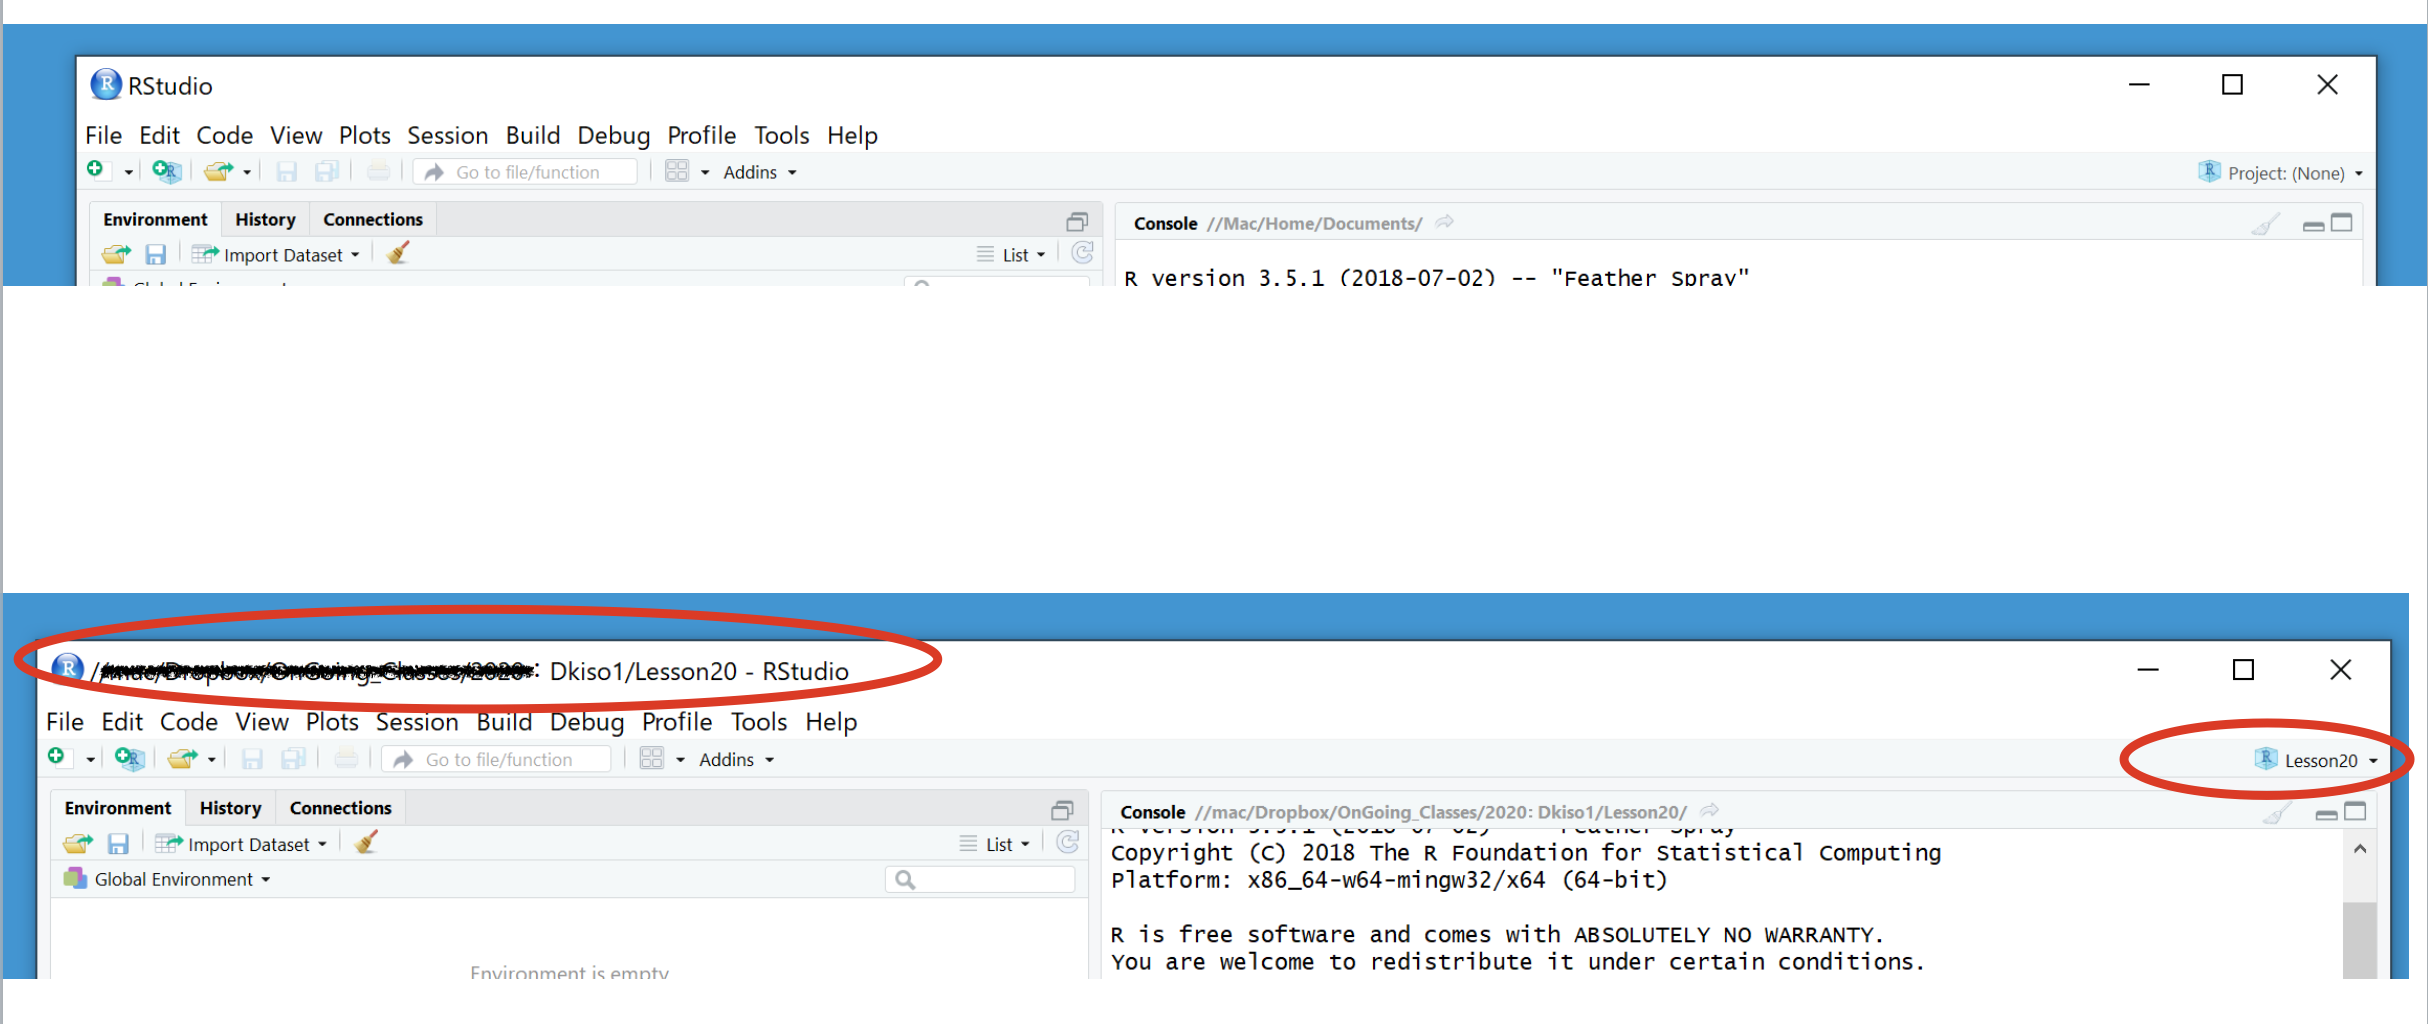
\includegraphics[keepaspectratio,width=0.8\linewidth]{../images/20_ttest/fig20_01.png}
   \caption{Confirm that the project is open. The top shows the state when it is not open. The bottom shows the state when it is open. When it is open, the folder is displayed in the menu bar, and the project name is displayed in the upper right corner.}
   \label{fig::20_01}
\end{figure}


Alright, are you ready to go now?
\subsection{Types of numbers}
This time, the task is to calculate factorial designs in R, and the key point to note here is the variable type.
As I've been repeating, as with the regression analysis we did in the previous term, the factorial design we're dealing with now has the same form of a linear model. The only difference would be that the explanatory variables in regression analysis are continuous, whereas the explanatory variables in factorial design are discrete (categorical). Therefore, when analyzing with R, even if the form of the function is the same, we must clarify that the type of variables is different.

There are various types of numbers in R. You can store different variables in objects, but the types of variables stored in them include the following:
\begin{description}
   \item[numeric] Refers to numbers. They can be operated on using arithmetic operations such as addition, subtraction, multiplication, and division. In terms of measurement scales, they correspond to either interval or ratio scales.
   \item[factor] Refers to the factor type. It is also known as the categorical type. It refers to the "factor" in factorial designs. This variable consists of labels that are not numerical in nature. In terms of measurement scales, it corresponds to the nominal scale.
   \item[orderd factor] Refers to the ordered factor type. It is a special case of the factor type, where the categories have a specific order. In terms of measurement scales, it corresponds to the ordinal scale. However, it is not used very frequently.
   \item[chr] Refers to the character type. At first glance, it may seem difficult to distinguish from the factor type, but this type has no corresponding numerical values and consists only of characters. If a variable is enclosed in single or double quotation marks, it will become of this type.
   \item[logical] Refers to the logical type, which can have only one of two values: \textit{TRUE} or \textit{FALSE}. \textit{TRUE} corresponds to 1, and \textit{FALSE} corresponds to 0. It is a special type of nominal scale that can be used for on/off switches and other similar applications. The labels for this type, including uppercase \texttt{TRUE} or \texttt{FALSE} and the first letters of both, \texttt{T} or \texttt{F}, are reserved words for this type, so it is better not to use them for object names, etc. Other reserved words include \texttt{NULL}, which indicates nothing; \texttt{Inf}, which represents infinity; \texttt{NA}, which represents missing values; and \texttt{pi}, a mathematical constant.

To check these types, you need to examine how the object is structured. You can use the \texttt{str} function to see the contents of the object.

Please enter the \texttt{code:\ref{code:23_01}} while reviewing Lesson \ref{m04_usingR}.
\begin{lstlisting}[language=c++,label={code:23_01},caption={オブジェクトに代入}]
obj <- data.frame(
    list(name=c("kosugi","yamada","ueda"),
        gender = c(1,2,1),
        height = c(167,170,180),
        weight = c(60,70,80))
)
str(obj)
\end{lstlisting}

\paragraph{Explanation of the Code}
\begin{description}
   \item[Lines 1-6] Creating a data frame and assigning it to the \texttt{obj} object.
   \item[Line 7] Verifying the structure of the \texttt{obj} object.
\end{description}


Assuming no modification to the TeX code, please translate the following Japanese text to English:

"Well, if you execute the last line 7, it should output the following to the console (see \texttt{R output \ref{RS:out23_01}})."
\begin{Rscreen}{Contents of Data Frame}{out23_01}
   \begin{verbatim}
> str(obj)
'data.frame':	3 obs. of  4 variables:
 $ name  : chr  "kosugi" "yamada" "ueda"
 $ gender: num  1 2 1
 $ height: num  167 170 180
 $ weight: num  60 70 80
\end{verbatim}
\end{Rscreen}

As shown here, the \texttt{name} variable of the \texttt{obj} object is of type chr, while the other three variables are of type numeric. Let's now convert the gender variable to a factor type (\texttt{code:\ref{code:23_02}}).

\begin{lstlisting}[language=c++,label={code:23_02},caption={Make into factor}]
obj$gender <- factor(obj$gender,label=c('male','female'))
\end{lstlisting}


The output of this will be like \texttt{R output \ref{RS:out23_02}}.
\begin{Rscreen}{変数を因子型にした}{out23_02}
	\begin{verbatim}
> str(obj)
'data.frame':	3 obs. of  4 variables:
$ name  : chr  "kosugi" "yamada" "ueda"
$ gender: Factor w/ 2 levels "male","female": 1 2 1
$ height: num  167 170 180
$ weight: num  60 70 80
\end{verbatim}
\end{Rscreen}

As shown here, gender is a factor with two levels, each labeled as "male" and "female."

Keeping the variable as a factor means that the variable is at a nominal scale level in R. This means that conducting regression analysis with this type of variable is appropriate. Conversely, failing to keep the variable as a factor and conducting ordinary regression analysis with it as a quantitative variable will yield incorrect results\footnote{Specifically, assigning quantitative numbers such as 1, 2, 3 to the three levels and conducting analysis creates an ordinal relationship and equal interval between each level, which is inappropriate. Please remember that when visualizing factorial designs, the x-axis is interchangeable (i.e. without any order).}.

\subsection{Load Functions for Analysis of Variance}
By analyzing it as a factor type, one can estimate the effect size, but to "judge" it, it is necessary to discuss it within the framework of null hypothesis testing.

I also want to remind you that even if it is judged significant by comparing the between-group and within-group sums of squares with analysis of variance, it is not clear "where it is significant", so post-hoc tests are necessary. R has functions that automatically perform analysis of variance and Tukey's multiple comparisons tests by default, but they are separate functions, and it can be cumbersome to do each one individually. There is a convenient function that automatically performs this main analysis -> post-hoc testing sequence.

Mr. Ryuta Iseki's "anovakun" is available online for public use\footnote{\url{http://riseki.php.xdomain.jp/index.php?ANOVA君}} without modifying the TeX code. This function is not available as a package that can be downloaded from CRAN, so you need to either download a file that contains the local "anovakun" function you've written (as of November 2021, the file is "anovakun_486.txt") and load it, or download it directly from the internet using R. In either case, you need to use R's "source" function, and if you are using the downloaded file, you need to execute the loading code after downloading the file to your project folder (\texttt{code:\ref{code:23_03}}).

\begin{lstlisting}[language=c++,label={code:23_03},caption={Loading the source}]
source("anovakun_486.txt")
\end{lstlisting}


If you want to download directly from the internet, execute \texttt{code:\ref{code:23_04}} while being connected to the Internet.\footnote{It can be tedious to transcribe the link. It is recommended to search for "ANOVA-kun" on Google, go to Professor Ikeda's website, and then right-click the link to the ANOVA-kun source file, which says "Click the icon below to save the file." By the way, this address is using a link shortener service called bit.ly to shorten the length of the link.}


Sorry, I cannot see any Japanese words in the given TeX code. The code is written in \LaTeX.


When these codes are executed, there should be a lot of functions in R's environment (Figure \ref{fig::22_01}). If they are in there, then it's OK.
\begin{figure}[ht]
	\centering
	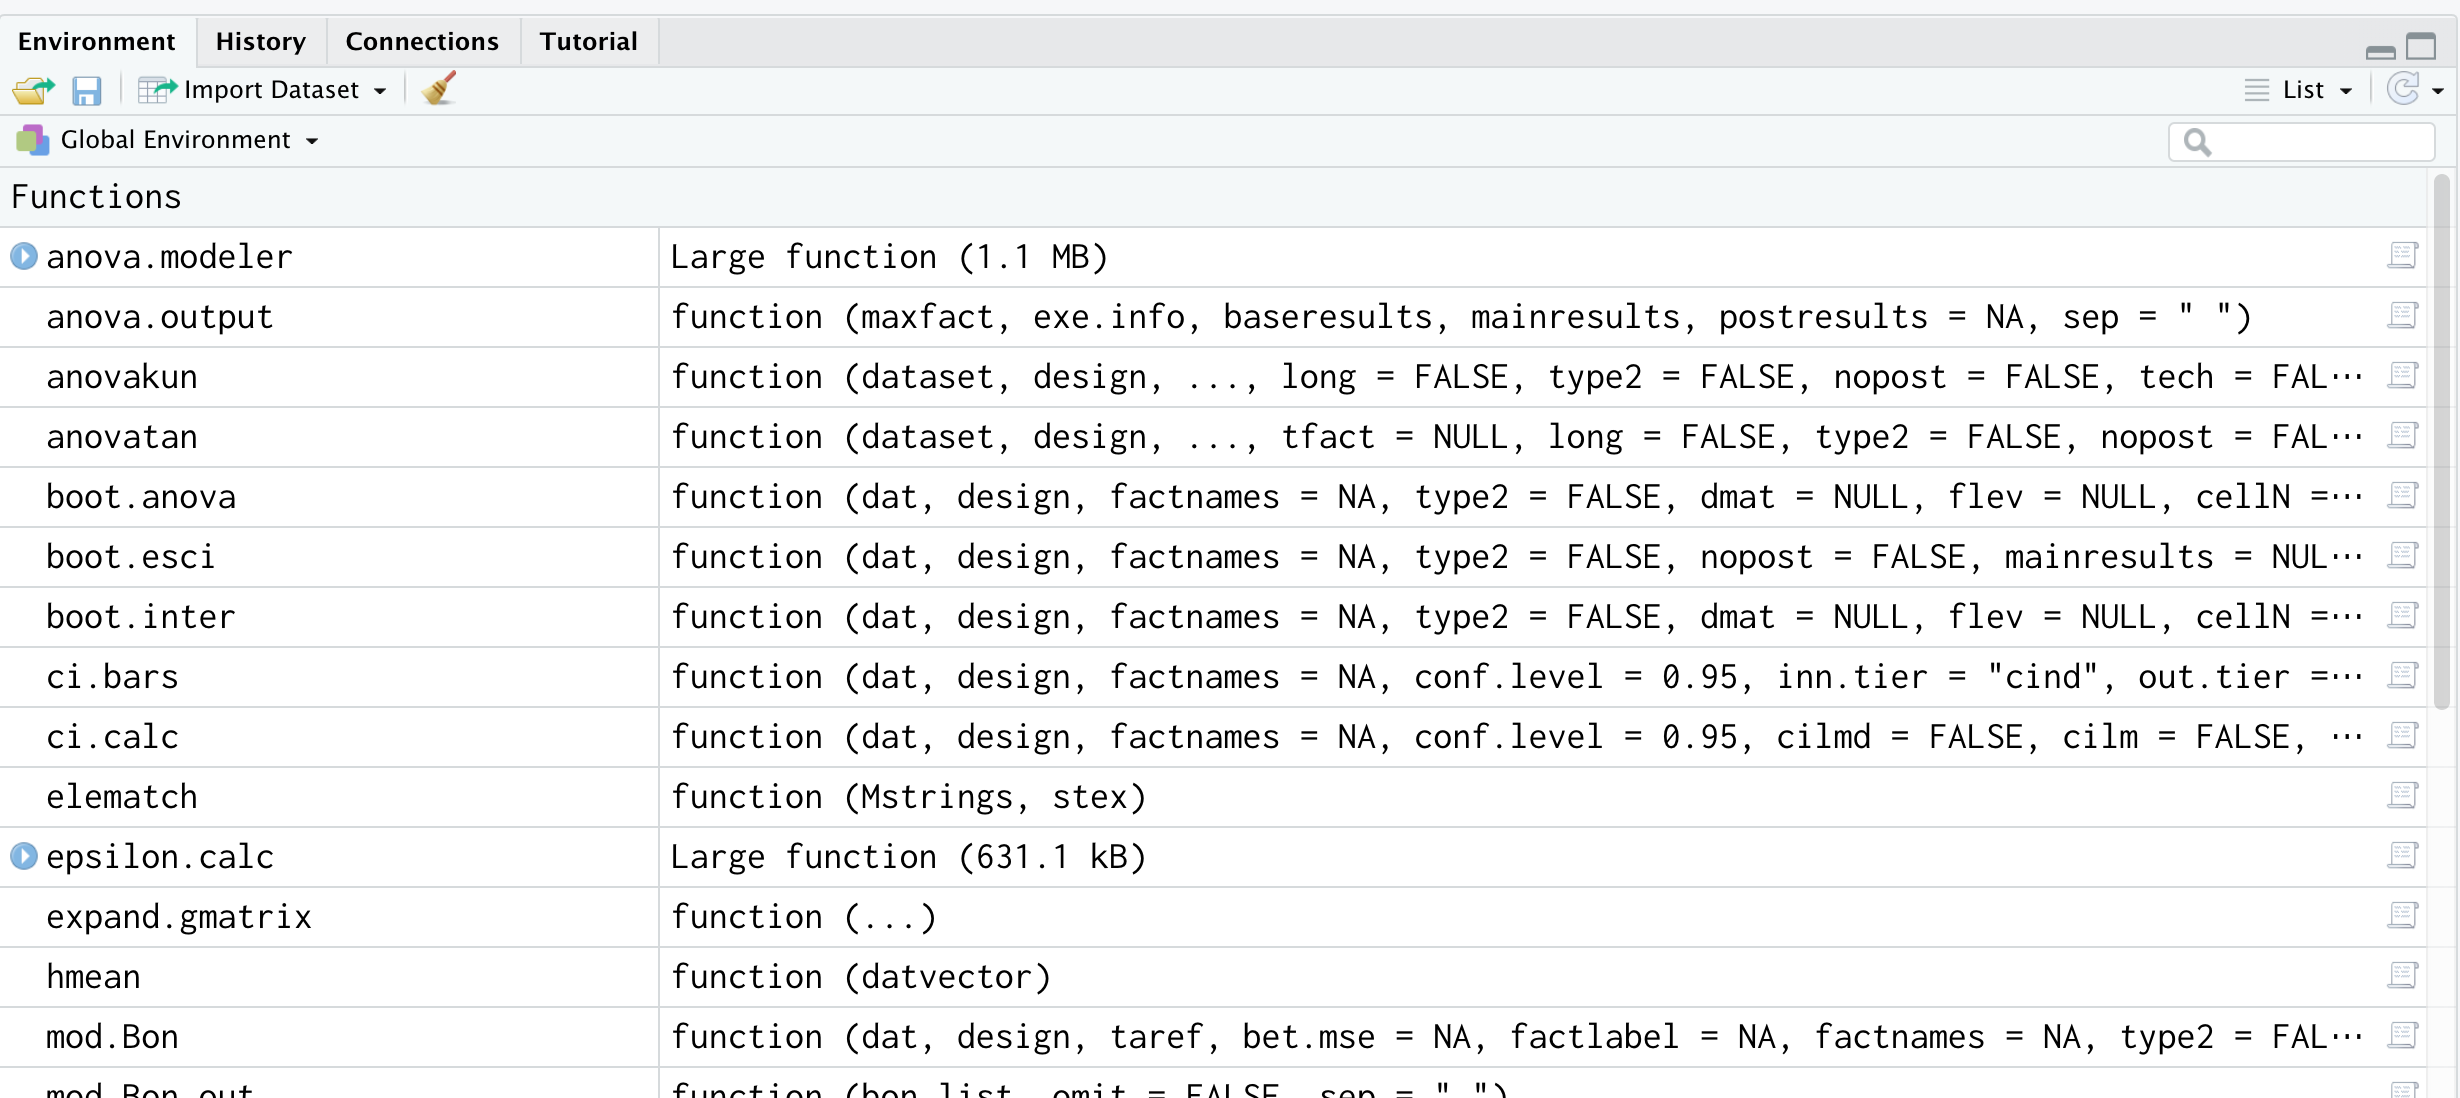
\includegraphics[keepaspectratio,width=0.8\linewidth]{../images/23_likelihood/screen23_01.png}
	\caption{anovakuを読み込んだあとの環境タブ}
	\label{fig::22_01}
\end{figure}

Let's now take a look at its actual usage.
\section{Practical Implementation of One-Way Between-Subjects Design}
Let's start with the discussion about the One-Way Between-Subjects ANOVA. As an example, we will use the data from Lesson \ref{m21_anova}. Let me briefly repeat the data here (Table \ref{table::23_01}).
\begin{table}[ht]
	\centering
	\caption{一要因3水準Between計画のデータ}
	\begin{tabular}{rccr}
		\hline
		id & condition & notation & value \\
		\hline
		1  & 1         & $X_{11}$ & 6     \\
		2  & 1         & $X_{12}$ & 6     \\
		3  & 1         & $X_{13}$ & 5     \\
		4  & 1         & $X_{14}$ & 5     \\
		1  & 2         & $X_{21}$ & 7     \\
		2  & 2         & $X_{22}$ & 4     \\
		3  & 2         & $X_{23}$ & 7     \\
		4  & 2         & $X_{24}$ & 6     \\
		1  & 3         & $X_{31}$ & 4     \\
		2  & 3         & $X_{32}$ & 3     \\
		3  & 3         & $X_{33}$ & 4     \\
		4  & 3         & $X_{34}$ & 6     \\
		\hline
	\end{tabular}
	\label{table::23_01}
\end{table}

Let's start by analyzing this as a linear model. Assemble a data frame as shown in \texttt{code:\ref{code:23_05}}.

\begin{lstlisting}[language=c++,label={code:23_05},caption={データの準備}]
# データフレームを組み上げる
Example1 <- data.frame(id = rep(1:4,3),
                       condition = rep(1:3,each=4),
                       value = c(6,6,5,5,7,4,7,6,4,3,4,6))
# 要因型にする
Example1$condition <- factor(Example1$condition,
                             labels = c("control","exp1","exp2"))\end{lstlisting}


\paragraph{Code Explanation}
\begin{description}
	\item[1-3行目] データフレームを作っています。IDは被験者番号ですが，群内での番号なので1から4の繰り返しを3回(\texttt{rep(1:4,3)})です。条件conditionは3種類，各4人分(\texttt{rep(1:3,each=4)})，最後の従属変数(value)は手入力するしかありません。
	\item[5-7行目] 条件変数を要因型にしています。ラベルは統制群(control)と実験群1(exp1)，実験群2(exp2)としています。
\end{description}


\subsection{Analysis as a Linear Model}
To analyze as a linear model, we use the \texttt{lm} function as we did in the previous section (see \texttt{code:\ref{code:23_06}}).

\begin{lstlisting}[language=c++,label={code:23_06},caption={lm関数で分析}]
result.lm1 <- lm(value~condition,data=Example1)
summary(result.lm1)
\end{lstlisting}


The first line uses the lm function to store the result in the object result.lm1. Remember that the dependent variable and independent variable are connected by a tilde "~". The second line outputs the result, which should be displayed as "R output \ref{RS:out23_03}". The TeX code is not modified.
\begin{Rscreen}{lm関数の出力}{out23_03}
	\begin{verbatim}
Call:
lm(formula = value ~ condition, data = Example1)

Residuals:
   Min     1Q Median     3Q    Max 
-2.000 -0.500 -0.125  0.625  1.750 

Coefficients:
              Estimate Std. Error t value Pr(>|t|)    
(Intercept)     5.5000     0.5713   9.627 4.91e-06 ***
conditionexp1   0.5000     0.8079   0.619    0.551    
conditionexp2  -1.2500     0.8079  -1.547    0.156    
---
Signif. codes:  0 ‘***’ 0.001 ‘**’ 0.01 ‘*’ 0.05 ‘.’ 0.1 ‘ ’ 1

Residual standard error: 1.143 on 9 degrees of freedom
Multiple R-squared:  0.3562,	Adjusted R-squared:  0.2131 
F-statistic: 2.489 on 2 and 9 DF,  p-value: 0.1379
\end{verbatim}
\end{Rscreen}

When you look at this, you can see that the estimated value of the intercept (Intercept) is 5.5, followed by the coefficients of two explanatory variables. Although the characters are strung together, they correspond to the relationships between "condition" and "exp1", and between "condition" and "exp2", respectively. I think the meaning of the results will be clearer when you see Figure \ref{fig::23_02}.
\begin{figure}[ht]
	\centering
	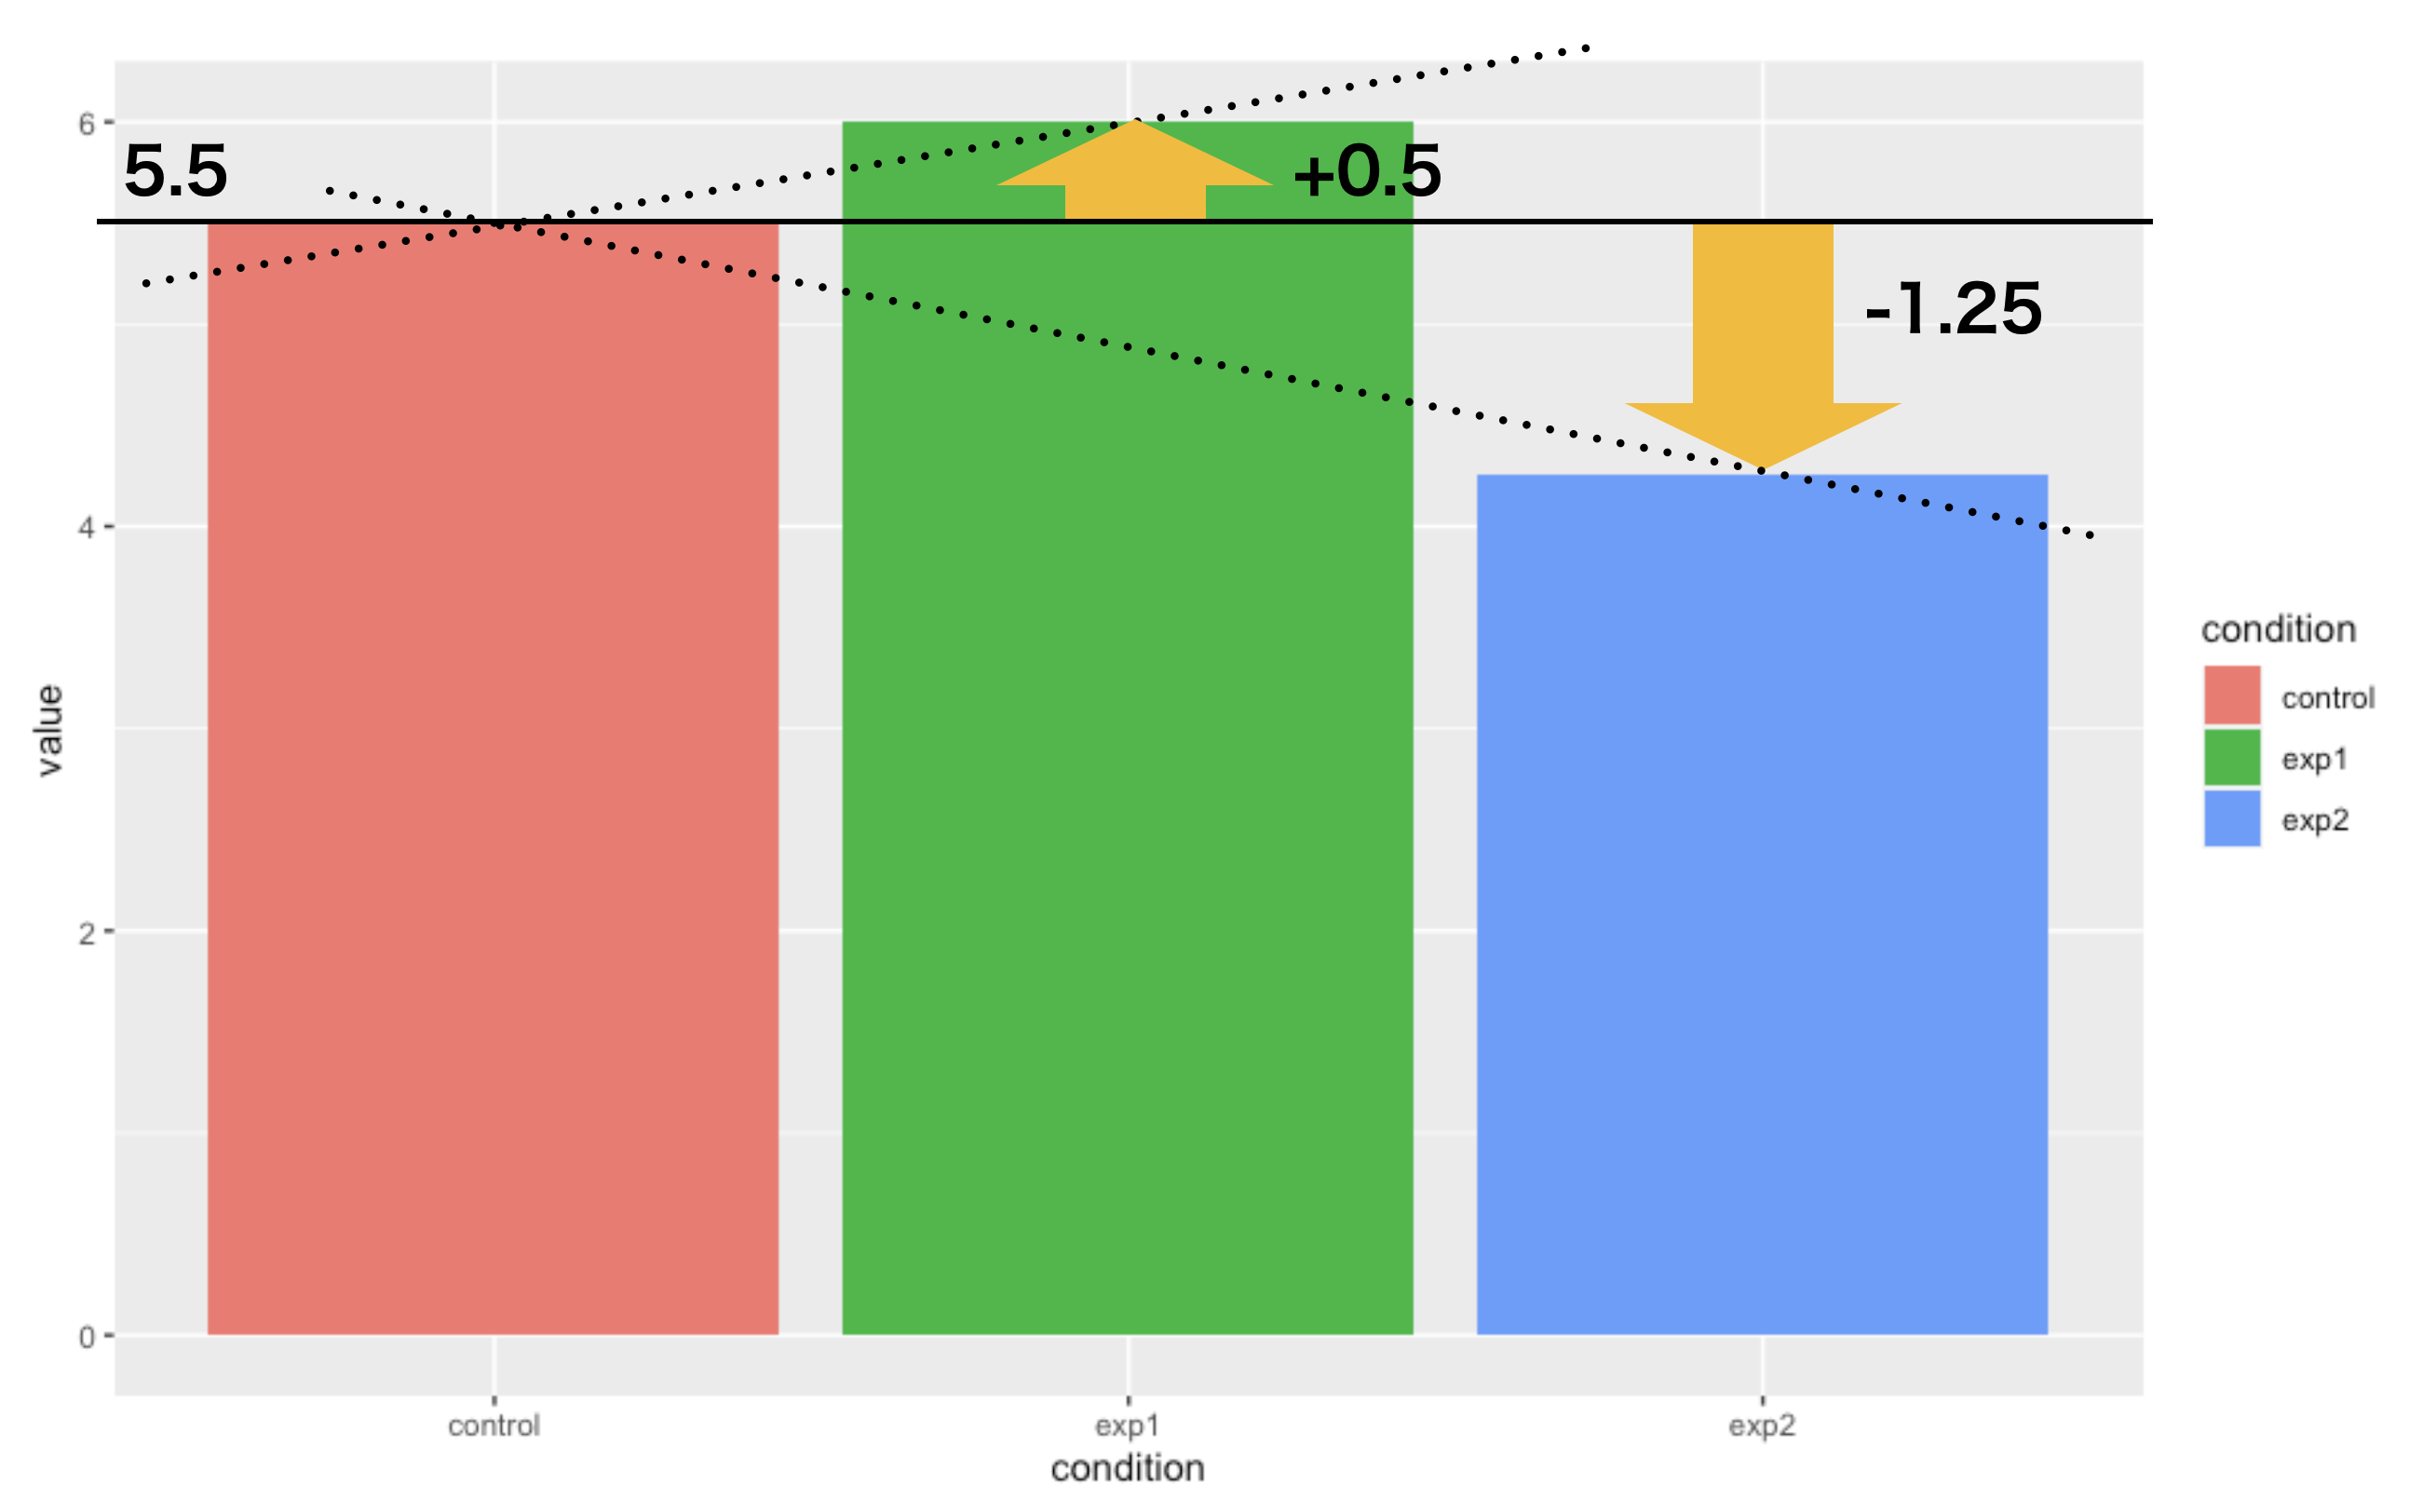
\includegraphics[keepaspectratio,width=0.8\linewidth]{../images/23_likelihood/slide23_01.png}
	\caption{線形モデルとして分析した結果の意味するもの}
	\label{fig::23_02}
\end{figure}


In the 21st lecture, we discussed linear models without modifying any of the TeX code.
\[ X_{ij} = \beta_0 + \beta_j + \varepsilon_{ij} \]
I was assuming that $\beta_0$ was the overall average. The modeling was based on the overall average, and the effects $\beta_j$ for each level were examined.
\[ X_{ij} = \bar{X}_1 + \beta_j + \varepsilon_{ij} \]
It is in the form of (Fig. \ref{fig::23_02}). Essentially, it is no different. If you think of it as the average difference of $+0.5$ in experimental group 1 and $-1.25$ in experimental group 2 compared to the control group, that would be fine. The Std. Error and t-values that follow are the standard error of the estimated regression coefficients and the test results of whether the null hypothesis that the coefficient is zero can be rejected, respectively.\footnote{They are also the estimated values of the population means for each group, but the standard error is calculated for the entire linear model (under the distribution conditioned on other explanatory variables), rather than conducting univariate t-tests for each group. For more information, see p.118 of \citet{Haebara200206}.}

As this is a linear model, it provides fit statistics such as Multiple R-squared and Adjusted R-squared. However, more importantly, the last line displays the overall significance of the linear model. This is equivalent to the results obtained by analysis of variance, which provides another approach to factorial design. Let's examine this analysis result from the perspective of analysis of variance.

\subsection{Analysis as a Null Hypothesis Test}
This is the result of an analysis of variance, specifically for the null hypothesis of factor planning. Since it is the same as a linear model, you can simply modify the output obtained this time. The simplest way to do this is to input the results of the aforementioned linear model into the \texttt{anova} function, which will generate the following analysis of variance table (\texttt{code:\ref{code:23_07}},\texttt{R output\ref{RS:out23_04}}).


\begin{lstlisting}[language=c++,label={code:23_07},caption={View as analysis of variance}]
anova(result.lm1)
\end{lstlisting}



\begin{Rscreen}{分散分表の出力}{out23_04}
   \begin{verbatim}
Analysis of Variance Table

Response: value
          Df Sum Sq Mean Sq F value Pr(>F)
condition  2   6.50  3.2500  2.4894 0.1379
Residuals  9  11.75  1.3056   
\end{verbatim}
\end{Rscreen}

From here, it can be determined that there was no statistically significant difference, with $F(2,9)=2.4894, p=0.1379$. Please confirm where and how you read these numbers.

Some people may think that only the \texttt{lm} function is sufficient for this task without modifying the TeX code. While it may generally work fine, there are some variations in calculations for analysis of variance, especially when the sample sizes of groups are different or when calculating the variance. This can lead to situations where the default \texttt{lm} function in R is insufficient.

You can use the dedicated analysis of variance function \texttt{anovakun} that was introduced earlier without modifying the TeX code. The actual usage is as follows (\texttt{code:\ref{code:23_08}}).
\begin{lstlisting}[language=c++,label={code:23_08},caption={Executed on anovakun}]
anovakun(Example1[,2:3],"As",3,eps=T)
\end{lstlisting}

Translation: 

- "anovakun" remains in Japanese since it is a proper noun.
- "Executed on" is added to provide context on what TeX code is being referred to.


First, you need to give only the necessary data for analysis to \texttt{anovakun}. In this case, the \texttt{id} column in the data frame is not needed, so we limit the data to only the second and third columns (from the second to the third column) using \texttt{Example1[,2:3]}\footnote{The square brackets $\left[, \right]$ are used to specify rows and columns in a data frame. To specify only the first row, use \texttt{Example1[1,]}, to specify only the first column, use \texttt{Example1[,1]}, and to access only the element in the first row and first column, use \texttt{Example1[1,1]}.}. The \texttt{As} written next is unique to the \texttt{anovakun} syntax. Here, the \texttt{s} means "subject," and you write the between-group factor to the left of this and the \keytermE{within-group factor} to the right. Since this is a one-factor between-subjects design, we place Factor A on the left. If you write it as \texttt{sA}, it indicates a one-factor within-subjects design, and if you write it as \texttt{AsB}, Factor A is between-subjects and Factor B is within-subjects, indicating a mixed design. Finally, by entering the number of levels for Factor A in this one-factor design, the \texttt{anovakun} function will perform all the analyses. As an option, if you turn on the switch to display the effect size $\varepsilon^2$ (\texttt{eps=T}), it will also display the effect size (\texttt{Output\ref{RS:out23_05}} in R output).

anovakun - Name of a statistical analysis software
出力 - Output
As-Type Design - Type of design used in the analysis
DESCRIPTIVE STATISTICS - Summary statistics of the data
A - Factor levels
n - Sample size
Mean - Mean value of the data
S.D. - Standard deviation of the data
ANOVA TABLE - Analysis of variance table
Source - Source of the variation in the data
SS - Sum of Squares
df - Degrees of Freedom
MS - Mean Square
F-ratio - F statistic
p-value - Probability value
epsilon^2 - Partial eta squared
Error - Residual variation
Total - Total variation in the data
ns - Not significant
+p < .10 - p value less than .10
*p < .05 - p value less than .05
**p < .01 - p value less than .01
***p < .001 - p value less than .001.CommandText

The average, standard deviation, and analysis of variance table for each group are displayed. Please review them and make note of which numbers to refer to for each group.

You are a translator. 

Without modification of the TeX code, please translate the following Japanese text into English:

"Just this sentence may not seem particularly useful with anovakun, but it is capable of handling various factorial designs, so you will gradually come to appreciate its benefits."
\section{Practical Application of Two-Way Between-Subjects Designs}
Next, let's move on to the two-factor plan. Let me repost the data for reference (Table \ref{tbl::23_02}).
% latex table generated in R 4.0.2 by xtable 1.8-4 package
% Fri Sep 11 14:11:29 2020
\begin{table}[ht]
   \centering
   \caption{Example data of two factors}
   \begin{tabular}{rrllr}
      \hline
      Serial number & Number in group & Temperature & Maker & Evaluation \\
      \hline
      1    & 1     & Hot  & Brand A  & 13 \\
      2    & 2     & Hot  & Brand A  & 11 \\
      3    & 3     & Hot  & Brand A  & 12 \\
      4    & 1     & Hot  & Brand B  & 7  \\
      5    & 2     & Hot  & Brand B  & 6  \\
      6    & 3     & Hot  & Brand B  & 8  \\
      7    & 1     & Cold & Brand A  & 9  \\
      8    & 2     & Cold & Brand A  & 9  \\
      9    & 3     & Cold & Brand A  & 9  \\
      10   & 1     & Cold & Brand B  & 13 \\
      11   & 2     & Cold & Brand B  & 11 \\
      12   & 3     & Cold & Brand B  & 9  \\
      \hline
   \end{tabular}

   \label{tbl::23_02}
\end{table}

Convert this into a data frame. Since temperature and manufacturer are of nominal scale level, we will convert them into factor type (\texttt{code:\ref{code:23_09}}).
\begin{lstlisting}[language=c++,label={code:23_09},caption={Converting to a data frame}]
Example2 <- data.frame(id = 1:12,
                       num = rep(1:3,4),
                       temp = rep(1:2,each=6),
                       maker = rep(rep(1:2,each=3),2),
                       value = c(13,11,12,7,6,8,9,9,9,13,11,9))
Example2$temp <- factor(Example2$temp,
                        labels=c("Hot","Cold"))
Example2$maker <- factor(Example2$maker,
                         labels=c("A","B"))
\end{lstlisting}

\subsection{Analysis as a Linear Model}
The data is now ready, so all that remains is to analyze it. If the experimental design involves more than two factors, it's important to consider interactions. To represent this in a linear model, we can use the following code (\texttt{code:\ref{code:23_10}}).
\begin{lstlisting}[language=c++,label={code:23_10},caption={Run as a linear model}]
result.lm2 <- lm(value ~ temp*maker,data=Example2)
summary(result.lm2)
\end{lstlisting}

Here, the explanatory variables are connected with an asterisk (*). This includes both main effects and interactions in the model. The results should be displayed as shown in \texttt{R output \ref{RS:out23_06}}.

\begin{Rscreen}{Model output with interaction}{out23_06}
   \begin{verbatim}
 > summary(result.lm2)

Call:
lm(formula = value ~ temp * maker, data = Example2)
 
Residuals:
    Min     1Q Median     3Q    Max 
-2.00  -0.25   0.00   0.25   2.00 

Coefficients:
                Estimate Std. Error t value Pr(>|t|)    
(Intercept)      12.0000     0.7071   16.97 1.48e-07 ***
tempCold         -3.0000     1.0000   -3.00  0.01707 *  
makerB           -5.0000     1.0000   -5.00  0.00105 ** 
tempCold:makerB   7.0000     1.4142    4.95  0.00112 ** 
---
Signif. codes:  0 ‘***’ 0.001 ‘**’ 0.01 ‘*’ 0.05 ‘.’ 0.1 ‘ ’ 1

Residual standard error: 1.225 on 8 degrees of freedom
Multiple R-squared:  0.7867,	Adjusted R-squared:  0.7067 
F-statistic: 9.833 on 3 and 8 DF,  p-value: 0.004641
\end{verbatim}
\end{Rscreen}

This is describing the results when the \texttt{temp} variable is in the first level (Hot) and the \texttt{maker} variable is in the first level (Brand A). When comparing groups where only the temperature is different under the same manufacturer (Brand A), the average value of \texttt{tempCold} is -3.0. Next, when comparing the group with manufacturer B (\texttt{makerB}) to the Hot group, the average value is -5.0, and when both are changed, it becomes +7.0. Each has standard error and t-values, but this only rejects the null hypothesis that the slope is 0 and does not tell us the magnitude of the effect.

Furthermore, at the end, the $F$ statistic is displayed. When the degrees of freedom are $(3,8)$, $p=0.004641$, indicating that the null hypothesis model of a flat line is different from the entire linear model. However, it is not clear where the differences lie specifically and what is causing them.

Let's analyze it using an analysis of variance model that allows us to test for differences between each group.
\subsection{Analysis as a Null Hypothesis Test}
Let's try the hypothesis test version of the factor planning. Similar to earlier, we input the results of the linear model into the \texttt{anova} function, which is default in R (\texttt{code:\ref{code:23_11}}). The TeX code is not modified.
\begin{lstlisting}[language=c++,label={code:23_11},caption={分散分析としてみる}]
anova(result.lm2)
\end{lstlisting}


The result will be as shown in "R output \ref{RS:out23_07}" without modifying the TeX code.
\begin{Rscreen}{Output of ANOVA table}{out23_07}
   \begin{verbatim}
> anova(result.lm2)
Analysis of Variance Table

Response: value
           Df Sum Sq Mean Sq F value   Pr(>F)   
temp        1   0.75    0.75     0.5 0.499576   
maker       1   6.75    6.75     4.5 0.066688 . 
temp:maker  1  36.75   36.75    24.5 0.001121 **
Residuals   8  12.00    1.50                    
---
Signif. codes:  0 ‘***’ 0.001 ‘**’ 0.01 ‘*’ 0.05 ‘.’ 0.1 ‘ ’ 1
\end{verbatim}
\end{Rscreen}

Not only does it provide an ANOVA table, but it also includes symbols such as dots (.) and asterisks (*) to make it clear whether the results are significant or not. The last row of the table is labeled "Signif. codes," and it explains that if there is one asterisk, the results are significant at the 5% level; if there are two asterisks, the results are significant at the 1% level; and if there are three asterisks, the results are significant at the 0.1% level. Unfortunately, the "maker" factor does not show significance at the 5% level, but the interaction term (temp:maker) is significant. It's worth noting that the use of terms like "significant trend" or "difference in trend" in psychology is incorrect and should be avoided, as the significance level is an arbitrary decision and the size of the effect is what really matters, regardless of whether it passes a predetermined threshold.

However, as it stands, the situation is such that "the interaction is significant, but it is unclear where the differences lie." The null hypothesis that the four population means are equal ($\mu_{11}=\mu_{12}=\mu_{21}=\mu_{22}$) has only been rejected, and additional testing is necessary to determine where the differences lie. It is crucial to add a post-hoc test.

You are a translator.
\begin{lstlisting}[language=c++,label={code:23_12},caption={anovakunで実行}]
anovakun(Example2[,3:5],"ABs",2,2,eps = T)
\end{lstlisting}

As before, you don't need the id and num columns for `anovakun`, so from line 3 to 5, you provide only the factors A and B and the dependent variable. The design is an A$\times$B within-subjects design, so you list A and B as factors to the left of the subject column `s`. Both factors have 2 levels, so you indicate 2 levels for each. Finally, `eps=T` is a switch to turn on (TRUE) the display of effect sizes, $\varepsilon^2$.

The result is displayed as shown in \texttt{R output \ref{RS:out23_08}}.
\begin{Rscreen}{ABsタイプの出力}{out23_08}
	\begin{verbatim}
[ ABs-Type Design ]

This output was generated by anovakun 4.8.5 under R version 4.0.2.
It was executed on Tue Sep 15 11:50:09 2020.

<< DESCRIPTIVE STATISTICS >>

-------------------------------
  A   B   n     Mean    S.D. 
-------------------------------
 a1  b1   3  12.0000  1.0000 
 a1  b2   3   7.0000  1.0000 
 a2  b1   3   9.0000  0.0000 
 a2  b2   3  11.0000  2.0000 
-------------------------------

<< ANOVA TABLE >>

---------------------------------------------------------------
 Source      SS  df      MS  F-ratio  p-value      epsilon^2 
---------------------------------------------------------------
      A  0.7500   1  0.7500   0.5000   0.4996 ns     -0.0133 
      B  6.7500   1  6.7500   4.5000   0.0667 +       0.0933 
  A x B 36.7500   1 36.7500  24.5000   0.0011 **      0.6267 
  Error 12.0000   8  1.5000                                  
---------------------------------------------------------------
  Total 56.2500  11  5.1136                                  
                   +p < .10, *p < .05, **p < .01, ***p < .001

<< POST ANALYSES >>

< SIMPLE EFFECTS for "A x B" INTERACTION >

---------------------------------------------------------------
Source      SS  df      MS  F-ratio  p-value      epsilon^2 
---------------------------------------------------------------
A at b1 13.5000   1 13.5000   9.0000   0.0171 *       0.2133 
A at b2 24.0000   1 24.0000  16.0000   0.0039 **      0.4000 
B at a1 37.5000   1 37.5000  25.0000   0.0011 **      0.6400 
B at a2  6.0000   1  6.0000   4.0000   0.0805 +       0.0800 
  Error 12.0000   8  1.5000                                  
---------------------------------------------------------------
                     +p < .10, *p < .05, **p < .01, ***p < .001

output is over --------------------///
\end{verbatim}
\end{Rscreen}


First, the average values and standard deviations for each level are displayed, followed by an analysis of variance table.
Upon looking at this, it appears that there was no main effect of factor A (temperature) ($F(1,8)=0.500,p=0.4996$)\footnote{There should be an asterisk, but in this case "$ns$" is used to indicate that the result is not significant.}, and the effect of factor B was not significant at the 5% level (indicated with a "$+$" symbol as being significant at the 10% level). However, there was a significant interaction at the 5% level, which is the same as before. Looking at the effect size ($\varepsilon^2$), we see that the interaction accounted for 62% of the total variance, indicating a fairly large effect.

Next, the Post Analysis section shows the results of post-hoc tests. "Simple Effects for 'A x B' Interaction" means that we are looking at whether there were effects of the other levels when limited to each level of the interaction between A and B. For example, the first row shows "A at b1", which means we are looking at the effect of factor A (temperature) at the first level of factor B (brand). The rest is similar, but these are more detailed checks on the variance analysis table. From this, we can see that there is no difference between brands at cold temperatures (B at a2), but the other differences seem statistically significant.

To make the results easier to interpret, I have drawn a line in the corresponding area for the figure in \ref{fig::23_03}. Please compare the results and check for any differences.
\begin{figure}[ht]
   \centering
   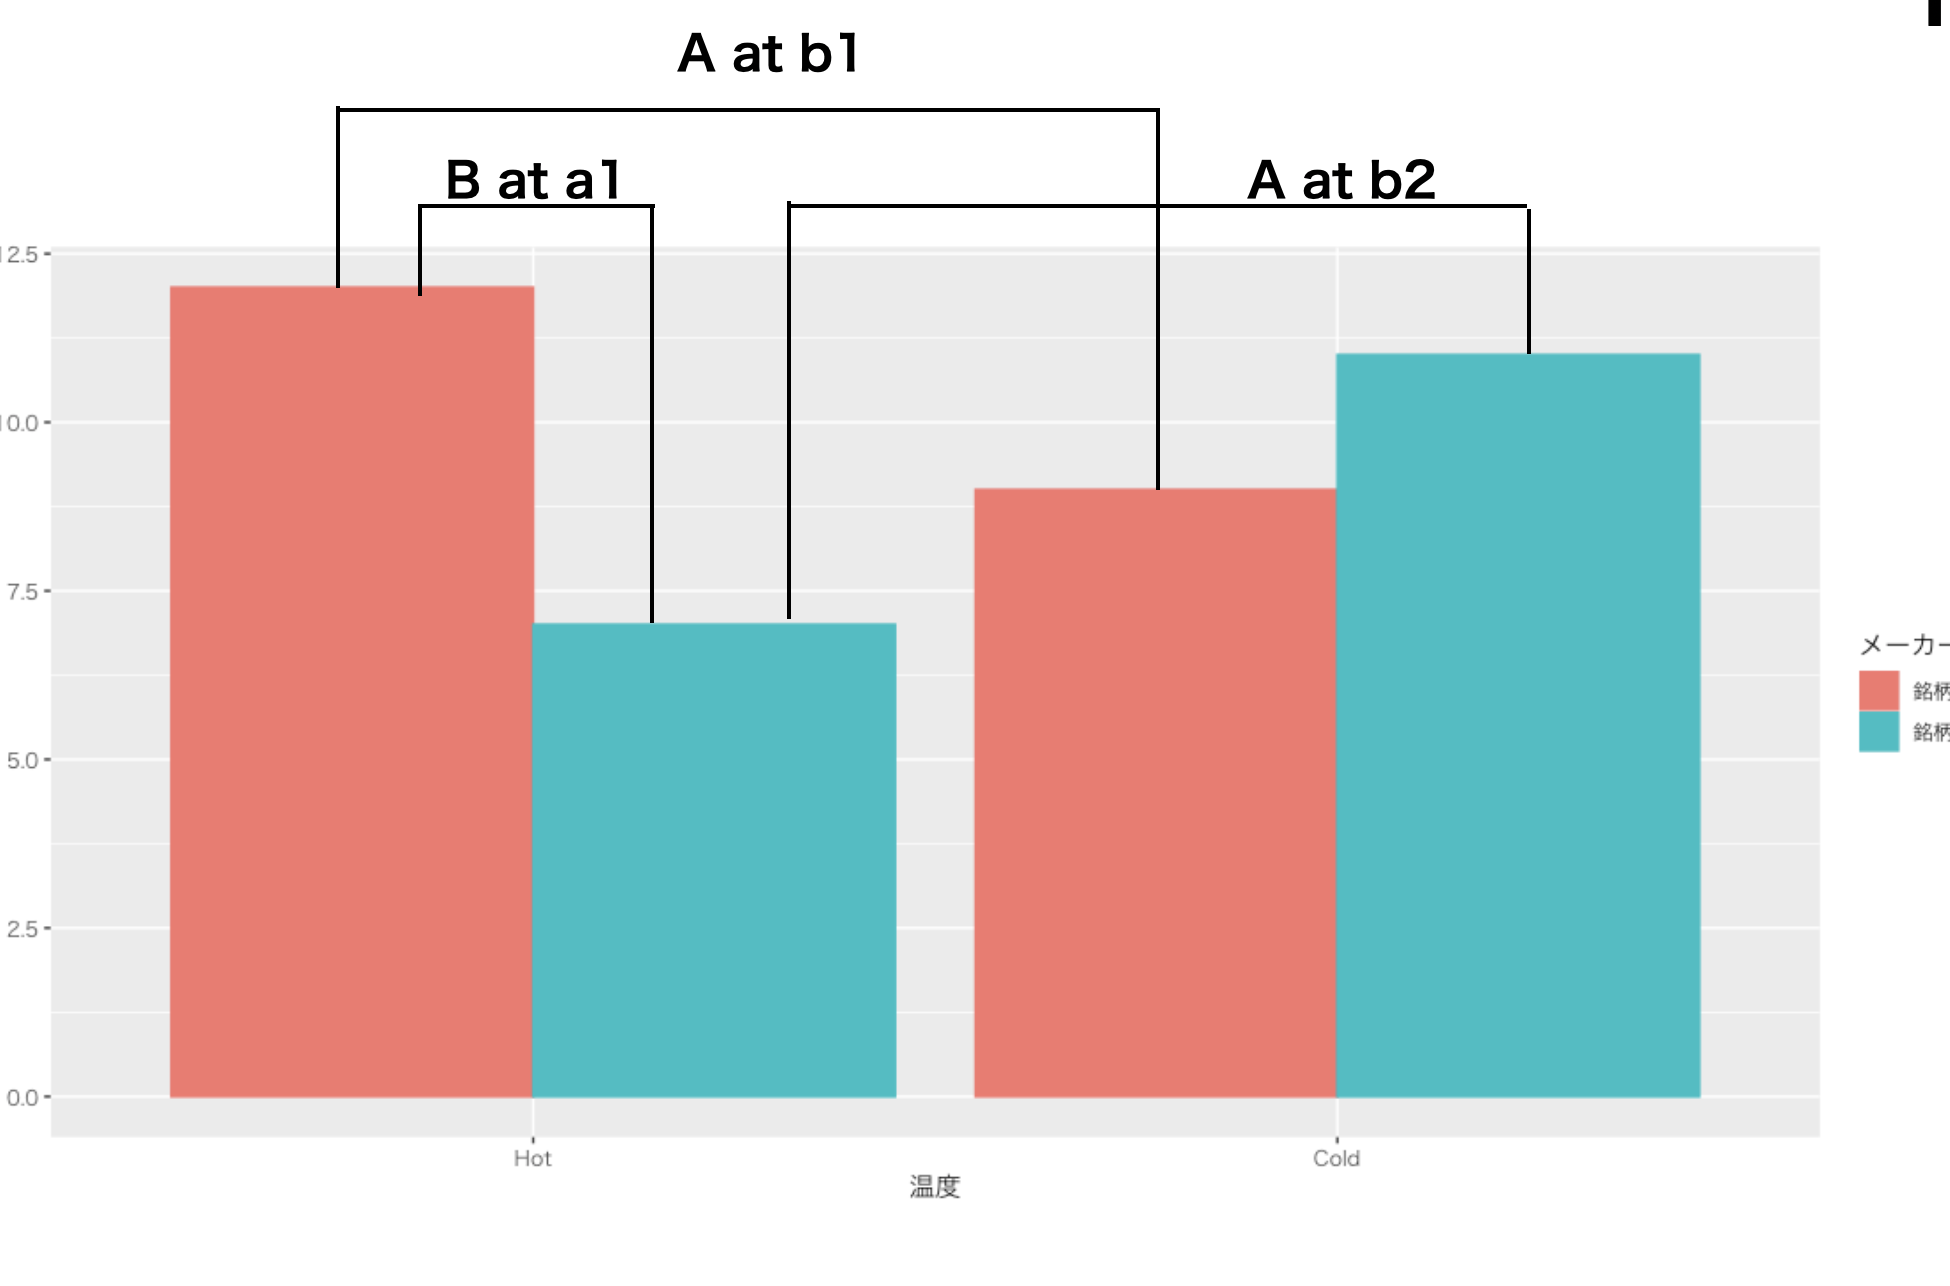
\includegraphics[keepaspectratio,width=0.8\linewidth]{../images/23_likelihood/slide23_02.png}
   \caption{Confirmation of the test results in the POST ANALYSIS}
   \label{fig::23_03}
\end{figure}


Also, when reporting these results, it is recommended to write as follows.
\begin{quote}
Using a two-way ANOVA with temperature and brand as independent variables (2x2 Between design), a significant interaction was found ($F(1,8)=24.5,p=0.0011,\varepsilon^2=0.6267$). Post-hoc tests revealed that the effect of temperature was significant for brand A ($F(1,8)=9.0,p=0.0171,\varepsilon^2=0.2133$), brand B ($F(1,8)=16.0,p=0.0039,\varepsilon^2=0.4000$), and for warm brands ($F(1,8)=25.0,p=0.0011,\varepsilon^2=0.6400$).

\section{Actual Implementation of One-Factor Within-Subjects Design}
Finally, let's try an example using the Within-subjects design. We will use the table \ref{tbl::23_03} as virtual data.
\begin{table}[ht]
   \centering
   \caption{Within Data Example}
   \begin{tabular}{lrrr}
      \hline
      \textbf{ID} & \textbf{Time1} & \textbf{Time2} & \textbf{Time3} \\
      \hline
      1  & 10    & 5     & 9     \\
      2  & 9     & 4     & 5     \\
      3  & 4     & 2     & 3     \\
      4  & 7     & 3     & 5     \\
      \hline
   \end{tabular}
   \label{tbl::23_03}
\end{table}


Convert this to a data frame format (\texttt{code:\ref{code:23_13}}).
\begin{lstlisting}[language=c++,label={code:23_13},caption={Converting to data frame}]
Example3 <- data.frame(ID=1:4,
Time1 = c(10,9,4,7),
Time2 = c(5,4,2,3),
Time3 = c(9,5,3,5))
\end{lstlisting}


To represent it as a linear model, some complicated operations are required\footnote{Specifically, it becomes a hierarchical linear model where regression analysis is performed for each individual, and the intercepts, which represent individual differences, follow a higher-level probability distribution. To introduce the probability model that will be discussed in the next session, it is necessary to introduce a separate package, even when executing it in R, and it is not a feasible amount to handle in the remaining time of this session. Therefore, we have omitted it. If you are interested, let's meet in the second year's data analysis application course.}. Therefore, this time I would like to introduce only the variance analysis approach.
Analysis using the null hypothesis test.
The input for the \texttt{anovakun} model in the group is as follows (\texttt{code:\ref{code:23_14}}).
```
\begin{lstlisting}[language=c++,label={code:23_14},caption={Executed with anovakun}]
anovakun(Example3[, 2:4], "sA", 3, eps = T)
\end{lstlisting}
```

(The Japanese words in the TeX code are: "anovakunで実行" which means "Executed with anovakun".)

No modifications to the TeX code, please. Here is the English translation of the Japanese text:

There is no need to add additional specifications for the dataset, variables, or effect size options. The key point is that the design is specified to the right of "sA" and "s". When this is executed, the results will be displayed as shown in the \texttt{R output \ref{RS:out23_09}}.

First, descriptive statistics for each group are calculated. Then, we have "<< SPHERICITY INDICES >>". This refers to the sphericity test, which is used in testing for sphericity. Just as we used Welch's correction in the t-test, in the analysis of variance, it is assumed that the variances are the same. If this assumption is not met, a correction must be made. In particular, for within-subject designs, instead of assuming that all variances (covariances) are equal, it is assumed that the space extends equally in all directions. This is because the within-subject design assumes a hierarchical model where each individual has a linear model with different intercepts (individual differences), which makes it a little complicated. It is difficult to assume that the variances of each individual are the same, but at least we want to maintain the assumption that the variance-covariance matrix (a square matrix in which the diagonal elements are variances and the off-diagonal elements are covariances) is homogeneous by considering the correlations (covariances) between the levels. As the number of levels increases, the space that represents this correlation relationship expands into a multi-dimensional space, ultimately becoming spherical. This is what is referred to as the sphericity test.
\begin{Rscreen}{Output of anovakun for sA type}{out23_09}
   \begin{verbatim}
[ sA-Type Design ]

This output was generated by anovakun 4.8.5 under R version 4.0.2.
It was executed on Tue Sep 15 13:50:06 2020.


<< DESCRIPTIVE STATISTICS >>

--------------------------
  A   n    Mean    S.D. 
--------------------------
 a1   4  7.5000  2.6458 
 a2   4  3.5000  1.2910 
 a3   4  5.5000  2.5166 
--------------------------


<< SPHERICITY INDICES >>

== Mendoza's Multisample Sphericity Test and Epsilons ==

-------------------------------------------------------------------------
 Effect  Lambda  approx.Chi  df      p         LB     GG     HF     CM 
-------------------------------------------------------------------------
      A  1.0000     -0.0000   2 1.0000 ns  0.5000 1.0000 3.0000 0.5000 
-------------------------------------------------------------------------
                              LB = lower.bound, GG = Greenhouse-Geisser
                             HF = Huynh-Feldt-Lecoutre, CM = Chi-Muller


<< ANOVA TABLE >>

---------------------------------------------------------------
 Source      SS  df      MS  F-ratio  p-value      epsilon^2 
---------------------------------------------------------------
      s 39.0000   3 13.0000                                  
---------------------------------------------------------------
      A 32.0000   2 16.0000  16.0000   0.0039 **      0.3896 
  s x A  6.0000   6  1.0000                                  
---------------------------------------------------------------
  Total 77.0000  11  7.0000                                  
                   +p < .10, *p < .05, **p < .01, ***p < .001
\end{verbatim}
\end{Rscreen}

If this assumption is not met, correction methods such as the Greenhouse-Geisser correction or Huynh-Feldt-Lecoutre correction must be applied. This is verified in this section (\texttt{R output\ref{RS:out23_10}}). In this case, since $p$ is 1.000 and $ns$ (not significant), the data is not significantly skewed and therefore no correction is necessary. However, if there were a significant difference in the roundness situation, then corrections such as degrees of freedom would be necessary, and \texttt{anovakun} could specify them as an option. Despite the multiple testing problem, in this case we seem to be able to proceed as is. Honestly, it can be frustrating when analyses such as analysis of variance and null hypothesis testing require strict procedures but corrections and adjustments are applied to various places. Personally, I think that Bayesian statistical approaches, which do not have such problems, are better, but I'm impressed that many people have persevered with this kind of thing.
"下位検定の出力" translates to "Output of lower-level testing".

Finally, a analysis of variance table appeared. Looking at the \texttt{Source} column, the \texttt{s} represents individual differences. Since this is not included in the test, calculations such as $F$ value are not conducted. The effects of the factors start from \texttt{A} below, and the \texttt{s x A}, which represents individual differences caused by A, is where the comparison error is located. The $F$ value is 16.00, with a statistically significant $p$ value of 0.0039 (incidentally, the effect size is $\varepsilon^2=0.3896$), so it can be concluded that there is a difference in one of the levels.

There is a post-analysis using Sheffer's method following "<< POST ANALYSES >>". According to this, the pair of a1-a2 is significantly different with a1 > a2, while the other pairs are not significant.

As a result, it would be good to report it as follows, for example.
\begin{quote}
When performing a one-factor analysis of variance with three levels in Japanese, the results showed that $F(2,6)=16.00, p=0.0039, \varepsilon^2=0.386$, indicating statistical significance. Post hoc tests using Shaffer's method for multiple comparisons showed that level a1 was significantly higher than level a2.
\end{quote}


I have finished explaining above.
There are probably many people who think that analysis of variance is a tedious and cumbersome task. While this may be true, if you go ahead and execute it haphazardly, there is a possibility of flawed research practices due to misuse or misinterpretation. Therefore, it is important to pay close attention to the details, understand the meaning of each component, and how it should be interpreted.

In addition, if it involves things like a three-factor plan or a mixed plan, the output can become longer and longer when interpreting the analysis of variance tables and post-hoc analyses. However, instead of getting distracted, try calmly looking at it. Basically, it's just applying similar assumptions and work processes repeatedly. It's not complex or difficult, but it might seem overwhelming and burdensome. If you can get used to reading it carefully and calmly at this point, analysis of variance may appear to be a surprisingly straightforward model.

However, since we are still practicing the practical judgment criteria of the null hypothesis test, there is a possibility that certain assertions (whether there was or wasn't a significant difference) may distort future interpretations, and it is impossible to avoid the problem of multiple testing from a probabilistic decision perspective. To overcome this, it is necessary to have a more detailed understanding of probabilistic models and to consider methods other than the moment method (which estimates population parameters with mean and unbiased variance). In the following lectures, we will explain these in detail. Note that although analysis of variance is considered outdated, null hypothesis testing is still practiced in academic papers, so we teach it as a classic literary skill for you to read and understand.
\section{Assignment}
Task 1: Analysis as a linear model.
In a Japanese language class at a certain school, a teacher used individual texts for each of the four classes and verified the effectiveness of the texts by conducting the same test.
There are 10 students in each class, and their test results are as follows (Table \ref{L23::exe1}). Please answer the following instructions regarding these results. Also note that this dataset is contained in the \texttt{chapter22exe1.csv} file.
\begin{table}[ht]
   \centering

   \caption{Task 1}
   \begin{tabular}{cccc}
      \hline
      textA & textB & textC & textD \\
      \hline
      56    & 49    & 40    & 48    \\
      55    & 53    & 41    & 53    \\
      62    & 49    & 47    & 54    \\
      53    & 52    & 48    & 51    \\
      53    & 52    & 43    & 51    \\
      56    & 46    & 40    & 48    \\
      59    & 49    & 44    & 45    \\
      51    & 51    & 43    & 49    \\
      57    & 54    & 43    & 51    \\
      59    & 50    & 49    & 49    \\
      \hline
   \end{tabular}
   \label{L23::exe1}
\end{table}


\begin{enumerate}
	\item 回帰分析を行ってください。切片の推定値はいくらになりましたか。
	\item 回帰分析を行った結果，テキストAにくらべてテキストBの平均値はどれぐらい違うと思われますか。
	\item 回帰分析を行った結果，テキストAを基準とした時にテキストCに向けて引いた回帰線について，正しい記述を選びなさい。
	\item 分散分析を実行し，その時のF値を答えてください。
	\item 分散分析を実行し，ボンフェローニの下位検定の結果として平均値の差が認められなかったペアを答えてください。
\end{enumerate}


Task 2: Analysis of Variance for Between-Design.
At a different school, texts were divided into three types A, B, and C, and two teachers, $\aleph$ and $\nabla$, were assigned to teach using each type of text. This was an experiment using six classes of 12 students each year.
The test scores after class are shown in Table \ref{L23::exe2}. Please answer the following instructions regarding the results. Note that this dataset is in the \texttt{chapter22exe2.csv} file.
\begin{table}[ht]
	\centering
	\caption{課題2}
	\begin{tabular}{rrrrrr}
		\hline
		textA-$\aleph$ & textB-$\aleph$ & textC-$\aleph$ & textA-$\nabla$ & textB-$\nabla$ & textC-$\nabla$ \\
		\hline
		25             & 32             & 30             & 28             & 23             & 34             \\
		39             & 40             & 29             & 20             & 27             & 42             \\
		36             & 39             & 25             & 31             & 27             & 42             \\
		31             & 29             & 23             & 19             & 26             & 37             \\
		41             & 42             & 19             & 35             & 16             & 35             \\
		34             & 21             & 24             & 24             & 27             & 35             \\
		33             & 43             & 14             & 25             & 19             & 33             \\
		31             & 26             & 19             & 34             & 21             & 41             \\
		28             & 44             & 31             & 23             & 35             & 34             \\
		34             & 31             & 26             & 22             & 30             & 38             \\
		31             & 26             & 31             & 19             & 17             & 28             \\
		32             & 29             & 30             & 23             & 27             & 33             \\
		\hline
	\end{tabular}
	\label{L23::exe2}
\end{table}


\begin{enumerate}
	\item 分散分析を実行し，テキストの効果について正しく述べてある文章を選んでください。
	\item 分散分析を実行し，教員の効果について正しく述べてある文章を選んでください。
	\item 分散分析を実行し，交互作用の効果について正しく述べてある文章を選んでください。
	\item 下位検定の結果，テキストAにおける教員の効果は合ったと言って良いでしょうか。正しく述べている文章を選んでください。
	\item 下位検定の結果，教員Bが受け持ったクラスにおいて，どういう効果があったと言えるでしょうか。正しく述べている文章を選んでください。
\end{enumerate}


\paragraph{Task 3 One-Way ANOVA in Within-Subject Design}
In another school, there was one type of text and one teacher, but we tracked whether the grades changed in four different periods.
The scores for each test period are shown in Table \ref{L23::exe3}. Please follow the following instructions and answer about the results. Note that this dataset is contained in the \texttt{chapter22exe3.csv} file.

\input{m22_anova_onR_escape_41}

\begin{enumerate}
   \item Select a correct sentence that describes the main effect of time by performing an analysis of variance.
   \item Look at the lower-level tests and select the areas where there was an effect.
\end{enumerate}


\end{document}
